\section{Graphs}
\label{section:graphs}
In the study of algorithms, we often use graphs as an abstract structure to represent the fundamental algorithmic problem without distractions. For example, when you want to find the fastest route to walk to the study hall, or if you want the cheapest combination of flights to take you to Kuala Lumpur, then both questions are really the same problem. If we remove all the details that are unnecessary to solve the problem, like the names of the airports and whether we are walking or flying, then we end up with a graph. This section defines various concepts related to graphs, and \Cref{section:graph-problems} will formalize the underlying problem of this example as well as some other graph problems. Later, \Cref{section:planar-graphs} defines the concept of \emph{planar} graphs.

\begin{definition}[Graph]
    A \emph{graph} $G := (V, E, from, to)$ is given by
\begin{itemize}
    \item $V$, a collection of \emph{vertices}
    \item $E$, a collection of \emph{edges}
    \item $from : E \rightarrow V$, a mapping from each edge to its source vertex
    \item $to : E \rightarrow V$, a mapping from each edge to its target vertex 
\end{itemize}
\end{definition}

We also define the convenience function $reverse : E \rightarrow E$. For an edge $e \in E$, $reverse(e)$ is the edge going in the opposite direction, where $from(e) = to(reverse(e))$, and $to(e) = from(reverse(e))$.

If we are working with multiple graphs at once, say two graphs $G$ and $H$, then writing just $V$ is ambiguous. In such cases do we instead denote $V(G)$ and $V(H)$ as $G$'s and $H$'s vertices, respectively. The same goes for $E(G)$ and $E(H)$ for their edges.

\begin{definition}[Weighted graph]
    A \emph{weighted graph} $G := (V, E, from, to, weight)$ is a graph, where $weight : E \rightarrow \mathbb{R}$ is the \emph{weight} of each edge. If a graph is not weighted, we often treat it as if all edges have unit weight, a weight of 1. Algorithms intended for weighted graphs will therefore often work on unweighted graphs as well.
\end{definition}

\begin{definition}[Directed and undirected graphs]
    Let $G$ be a graph. $G$ is said to be an \emph{undirected graph} if each edge has an opposite: $\forall e \in E ~ \exists e' \in E : reverse(e) = e'$.
    If $G$ is not undirected, we say that $G$ is a \emph{directed graph}.
    Edges in directed graphs are often drawn as arrows, while edges in undirected graphs can be drawn using just a line.
\end{definition}

\begin{definition}[Neighbourhood]
    Let $G$ be a graph, and let $u \in V$ be a vertex in the graph. The \emph{neighbourhood} of $u$, denoted as $N(u)$, is defined as the vertices in $G$ that are reachable from $u$ using just a single edge: $N(u) := \{ to(e)  ~|~  e \in E, ~ from(e) = u\}$. 
    In code, it is usually more useful to consider neighbourhoods in terms of edges. We will therefore denote $G[u]$ as the edges in $G$ that start in $u$: $G[u] := \{e ~ | ~ e \in E, ~ from(e) = u\}$
    We also denote $deg(u) := |N(u)|$ as the size of $u$'s neighbourhood, often referred to as the \emph{degree} of $u$.
\end{definition}

\begin{definition}[Simple graph]
    Let $G$ be a graph. $G$ is said to be a \emph{simple} graph if for each pair of vertices $u,v \in V$, there exists \emph{at most} one edge $e$ such that $from(e) = u$ and $to(e) = v$. If two or more edges have the same endpoints, we say the edges are \emph{parallel} to each other, and that the graph has \emph{parallel} edges and is thus not simple.
\end{definition}

\begin{definition}[Sparse and dense graphs]
    Let $G := (V, E, from, to)$ be a graph, let $n := |V|$, and let $m := |E|$. We say that $G$ is a \emph{sparse} graph if $m \in O(n)$. On the contrary, we say that $G$ is a \emph{dense} graph if it is not sparse.
\end{definition}

\begin{definition}[Walk]
    A \emph{walk} $P := [e_1, e_2, ..., e_k]$ in a graph $G$, for $e_i \in E$, is a sequence of edges where each edge ends where the next one starts: $\forall i \in \{1,2,..,k-1\} : to(e_i) = from(e_{i+1})$.
    If $s := from(e_1)$ and $t := to(e_k)$, we say that $P$ is an \emph{$s$-$t$-walk} in $G$.
    Another way to denote a walk is to give a sequence of vertices in the order they are visited: $[u_1, u_2, ..., u_n]$, for $u_i \in V$. This works as long as the graph is simple, if there are multiple edges from $u_i$ to $u_{i+1}$, then the walk is ambiguous.
\end{definition}

\begin{definition}[Path]
    A \emph{path} $P := [e_1, e_2, ..., e_k]$ in a graph $G$ is a walk with the extra requirement that each vertex is used at most once: $\forall i, j \in \{1,2,..,k\} : j \neq {i+1} \rightarrow to(e_i) \neq from(e_j)$.
    If $s := from(e_1)$ and $t := to(e_k)$, we say that $P$ is path from $s$ to $t$, or an \emph{$s$-$t$-path} in $G$.
    Note that in some literature, a walk is referred to as a path, and a path is referred to as a \emph{simple} path. In this thesis, when we refer to paths they are always simple, meaning that they never repeat any vertices. If any vertices are repeated, we will refer to it as a walk.    
\end{definition}

\begin{definition}[Cycle]
    A \emph{cycle} in a graph is a walk that starts and ends in the same vertex. If it does not repeat any vertices except in the last verex, then we call is a \emph{simple cycle}.
\end{definition}

\begin{definition}[The cost of a walk]
    Let $P := [e_1, e_2, ..., e_k]$ be a walk in a weighted graph $G$. The \emph{cost} of $P$ is defined as the sum of the weights of its edges: $\sum_{i=1}^k weight(e_i)$. In a collection of walks, we say that the \emph{shortest} walk is the \emph{cheapest} one, the one with the lowest cost. Likewise for the longest and most expensive walk. 

    Note that in some literature, \emph{shortest} may instead mean \emph{fewest edges}, and the term \emph{length} could refer to both the number of edges and the cost. For that ambiguous reason, we will from now on avoid the word \emph{length}, and \emph{shortest} will always mean \emph{cheapest}. If a graph is unweighted, we pretend that all the edges have a unit weight of 1, and in that case the cost is the same as the number of edges.
\end{definition}

\begin{definition}[Components of a graph]
    Let $G$ be an undirected graph. A component in $G$ is a set of vertices of $G$ where all vertices in the component have paths to all other vertices in the component. Moreover, this must be a \emph{maximal} set: no other vertices in the graph can be added to the component without giving up this property.
\end{definition}

\begin{definition}[Connected graph]
    We say that an undirected graph is a \emph{connected} graph if it has exactly one component. If it hase more than that we call it a \emph{disconnected} graph, and if it has less it is an \emph{empty} graph.
\end{definition}

\begin{definition}[Cut]
    Let $G = (V, E, from, to)$ be a connected and undirected graph. A \emph{cut} $C \subseteq E$ of $G$ is a subset of edges such that $(V, E \setminus C, from, to)$ is a disconnected graph of exactly two components. If two vertices $s,t \in V$ end up in separate components after the cut, we denote $C$ as an $s$-$t$-\emph{cut} in $G$. See \Cref{figure:s-t-cut} for an example of an $s$-$t$-cut.
\end{definition}

\begin{figure}[H]
    \centering
    \begin{subfigure}{.45\textwidth}
        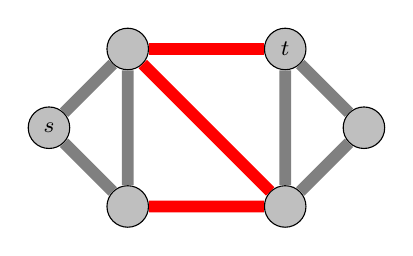
\begin{tikzpicture}
            \tikzstyle{every node}=[circle, fill=lightgray, draw=black, inner sep=2pt, minimum size=1.5em, font=\footnotesize, text=black]
            \tikzstyle{edge}=[gray, line width=1.5mm]
       
            \node (s) at (0,1) {$s$};
            \node (a) at (1,2) {};
            \node (b) at (1,0) {};
            \node (c) at (3,0) {};
            \node (d) at (4,1) {};
            \node (t) at (3,2) {$t$};

            \draw[edge] (s) -- (a) -- (b) -- (s);
            \draw[edge] (t) -- (d) -- (c) -- (t);
       
            \tikzstyle{edge}=[red, line width=1.5mm]
            \draw[edge] (b) -- (c) -- (a) -- (t);
        \end{tikzpicture}
        \caption{A connected graph with an $s$-$t$-cut marked in red}
        \label{subfigure:to-be-cut-graph}
    \end{subfigure}\hfill%
    \begin{subfigure}{.45\textwidth}
        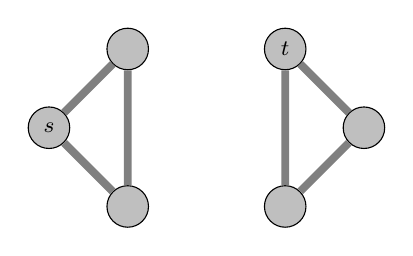
\begin{tikzpicture}
            \tikzstyle{every node}=[circle, fill=lightgray, draw=black, inner sep=2pt, minimum size=1.5em, font=\footnotesize, text=black]
            \tikzstyle{edge}=[gray, line width=1mm]
       
            \node (s) at (0,1) {$s$};
            \node (a) at (1,2) {};
            \node (b) at (1,0) {};
            \node (c) at (3,0) {};
            \node (d) at (4,1) {};
            \node (t) at (3,2) {$t$};

            \draw[edge] (s) -- (a) -- (b) -- (s);
            \draw[edge] (t) -- (d) -- (c) -- (t);
        \end{tikzpicture}
        \caption{The disconnected graph of exactly two components, after deleting all the edges in the cut}
        \label{subfigure:cut-graph}
    \end{subfigure}
    \caption{A graph before and after an $s$-$t$-cut of edges has been deleted}
    \label{figure:s-t-cut}
\end{figure}

% \begin{minipage}{.45\textwidth}
%     \begin{tikzpicture}
%         \tikzstyle{every node}=[circle, fill=lightgray, draw=black, inner sep=2pt, minimum size=1.5em, font=\footnotesize, text=black]
%         \tikzstyle{edge}=[gray, line width=1.5mm]
   
%         \node (s) at (0,1) {$s$};
%         \node (a) at (1,2) {};
%         \node (b) at (1,0) {};
%         \node (c) at (3,0) {};
%         \node (d) at (4,1) {};
%         \node (t) at (3,2) {$t$};

%         \draw[edge] (s) -- (a) -- (b) -- (s);
%         \draw[edge] (t) -- (d) -- (c) -- (t);
   
%         \tikzstyle{edge}=[red, line width=1.5mm]
%         \draw[edge] (b) -- (c) -- (a) -- (t);
%     \end{tikzpicture}
%     \captionof{A connected graph with an $s$-$t$-cut marked in red}
%     \label{subfigure:to-be-cut-graph}
% \end{minipage}\hfill%
% \begin{minipage}{.45\textwidth}
%     \begin{tikzpicture}
%         \tikzstyle{every node}=[circle, fill=lightgray, draw=black, inner sep=2pt, minimum size=1.5em, font=\footnotesize, text=black]
%         \tikzstyle{edge}=[gray, line width=1mm]
   
%         \node (s) at (0,1) {$s$};
%         \node (a) at (1,2) {};
%         \node (b) at (1,0) {};
%         \node (c) at (3,0) {};
%         \node (d) at (4,1) {};
%         \node (t) at (3,2) {$t$};

%         \draw[edge] (s) -- (a) -- (b) -- (s);
%         \draw[edge] (t) -- (d) -- (c) -- (t);
%     \end{tikzpicture}
%     \captionof{The disconnected graph of exactly two components, after deleting all the edges in the cut}
%     \label{subfigure:cut-graph}
% \end{minipage}